% Provenance (never printed): see sources/outline_sources.md (Year 2: the solar nebula
% and the condensation sequence; planetesimals and embryos; chondrites, achondrites and
% irons; the age of the Solar System; differentiation of planets). Curves from
% figdata/bachelor-2/nebula.py, condensation.py, al26.py, meteorites.py; exercise and
% problem values in the Book 4 scratch calculator calc/ch02.py.
\chapter{Planet Formation and Meteorites}\label{ch:b2:planet-formation-meteorites}

Every year some fifteen thousand tonnes of dust from space enter the Earth's
atmosphere; most of it burns up or settles as microscopic spherules, and once
in a while a stone the size of a fist falls with a fireball and a sonic boom.
Most of these stones are pieces of asteroids, and many have hardly changed
since they formed. Cut one open and polish it, and it shows millimetre-sized
beads of once-molten rock, white irregular grains of calcium and aluminium
minerals, flakes of metal, all held in a dark, fine-grained cement. The white
grains are the oldest solids of the Solar System: lead isotopes date them to
4567 million years. A second clock, the decay of a radioactive isotope of
aluminium that has long since vanished, dates the other components relative to
them to within a fraction of a million years. This chapter follows the disc of
the previous chapter as it turns into planets: which solids condense from the
cooling gas, and where; how dust grows into bodies kilometres across and then
into planets; what the \omterm{def:b2:planet-formation-meteorites:fall-find}{meteorites} are, and how they date these events; and why
some of the first bodies melted and grew iron cores while others stayed as they
had formed.
% ledger: rojas21:flux, lugaro:cai, gail:meteorites

\begin{recall}
Young stars are surrounded by \omterm{def:b2:ism-star-formation:disc}{protoplanetary discs}, which disappear within a
few million years; a grain in starlight at the distance $r$ from a star of
luminosity $L$ settles at $T = \bigl(L/(16\pi\sigma r^2)\bigr)^{1/4}$
(\cref{ch:b2:ism-star-formation}). Asteroids are the small rocky or metallic
bodies of the Solar System, most of which orbit between Mars and Jupiter (Year 1
volume). A radioactive nucleus decays with the probability $\lambda$ per unit
time: $N = N_0 e^{-\lambda t}$; the half-life is $\ln 2/\lambda$, and the mean
life $\tau = 1/\lambda$ (physics). In a closed system, cogenetic samples of
different parent-to-daughter ratios lie on a straight line, the isochron, whose
slope gives the age and whose intercept is the initial ratio (Year 1 volume).
Heating a mass $m$ of specific heat capacity $c$ by $\Delta T$ takes the energy
$mc\,\Delta T$ (physics).
\end{recall}

\section{The solar nebula}

\begin{definition}[Solar nebula]\label{def:b2:planet-formation-meteorites:nebula}
The \emph{solar nebula}\index{solar nebula} is the \omterm{def:b2:ism-star-formation:disc}{protoplanetary disc} of gas
and dust that surrounded the young Sun and from which the planets, their
satellites, the asteroids and the comets formed.
\end{definition}

How much matter did it hold? A lower limit comes from the planets themselves.
Add to each planet enough hydrogen and helium to give it the composition of the
Sun, spread the result over a ring centred on its orbit, and the surface
density, the mass per unit area of the disc, falls off with the distance from
the Sun. This reconstruction is the \emph{minimum-mass solar
nebula}\index{minimum-mass solar nebula}. In a widely used version the surface
density of the gas is
\[
  \Sigma_g = \qty{2200}{g.cm^{-2}}\left(\frac{r}{\qty{1}{au}}\right)^{-3/2},
\]
and that of the solids $\Sigma_p = \qty{33}{g.cm^{-2}}\,Z_{\mathrm{rel}}\,
(r/\qty{1}{au})^{-3/2}$, where $Z_{\mathrm{rel}}$ is the fraction of the
condensable matter actually solid: $0.33$ where only rock and metal have
condensed, about $0.78$ where water ice has joined them, $1$ beyond the place
where methane freezes. The numbers are uncertain: the heavy-element content of
Jupiter is known only to within a factor of four, and the planets need not have
formed where they orbit now.
% ledger: cy10:mmsn

\begin{proposition}[Mass of a disc]\label{prop:b2:planet-formation-meteorites:disc-mass}
A disc of surface density $\Sigma(r) = \Sigma_1 (r/r_1)^{-3/2}$ holds, inside
the radius $R$, the mass
\[
  M(R) = 4\pi\Sigma_1 r_1^2 \left(\frac{R}{r_1}\right)^{1/2}.
\]
Most of the mass lies far out: doubling the radius adds \qty{41}{\percent} to
the mass.
\end{proposition}

\begin{proof}
A ring of radius $r$ and width $\mathrm dr$ has the area $2\pi r\,\mathrm dr$, so
\[
  M(R) = \int_0^R 2\pi r\,\Sigma_1 \left(\frac{r}{r_1}\right)^{-3/2}\mathrm dr
       = 2\pi\Sigma_1 r_1^{3/2}\int_0^R r^{-1/2}\,\mathrm dr
       = 4\pi\Sigma_1 r_1^{3/2} R^{1/2},
\]
which is the formula; the integral converges at $r = 0$. Doubling $R$
multiplies $M$ by $\sqrt 2 = 1.41$.
\end{proof}

With $\Sigma_1 = \qty{2.2e4}{kg.m^{-2}}$ at $r_1 = \qty{1}{au}$, the minimum-mass
nebula holds $0.03$ solar masses inside \qty{100}{au} (\cref{exo:b2:planet-formation-meteorites:5}). The discs
observed around stars a million years old, weighed by the millimetre glow of
their dust, hold \numrange{0.001}{0.1} solar masses: the minimum-mass nebula
sits comfortably among them.
% ledger: cy10:mmsn

Almost all of this mass is gas that will never condense. The Sun was born
with a mass fraction of hydrogen $X_0 = 0.711$, of helium $Y_0 = 0.274$ and of
all heavier elements together only $Z_0 = 0.0149$. Cooling a gas of this
composition until everything that can freeze has frozen turns only
\qty{1.5}{\percent} of its mass into solids: \qty{0.49}{\percent} of rock and
metal, and \qty{1.0}{\percent} of ices of water, methane and ammonia, water ice
alone being \qty{0.57}{\percent}. All the rocky planets, and the cores of the
giants, were built from this small fraction.
% ledger: lodders:protosolar, lodders:condensates

The temperature of the disc decides what is solid where. A disc heated only by
its star, a \emph{passive} disc, is warm at its surface, where the grains see
the star directly (the proposition of \cref{ch:b2:ism-star-formation}), and
much colder in its midplane, which receives only the infrared re-emitted by
those surface grains. For a young star of one solar mass a model of such a disc
gives the midplane temperature
\[
  T = \qty{120}{K}\left(\frac{r}{\qty{1}{au}}\right)^{-3/7}.
\]
Accretion of gas through the disc, which releases gravitational energy, makes
the midplane hotter, especially early on and close to the star (figure below).
% ledger: cy10:passive

\begin{omfigure}
\begin{tikzpicture}
\begin{axis}[omrecord, width=0.82\linewidth, height=6.2cm, xmode=log, ymode=log,
  xmin=0.1, xmax=100, ymin=10, ymax=1000,
  xlabel={distance from the star $r$ (au)}, ylabel={temperature (K)},
  tick label style={font=\scriptsize}, label style={font=\small},
  legend pos=north east, legend style={font=\scriptsize, draw=black!30}]
\addplot[thick, red!70!black] table[x=r_au, y=T_grain] {figdata/out/bachelor-2-nebula-temp.dat};
\addlegendentry{grains in direct starlight}
\addplot[thick, blue!70!black] table[x=r_au, y=T_mid] {figdata/out/bachelor-2-nebula-temp.dat};
\addlegendentry{midplane of a passive disc}
\addplot[black!50, densely dashed, domain=0.1:100, samples=2] {182};
\addplot[black!50, densely dashed, domain=0.1:100, samples=2] {41};
\node[font=\scriptsize, anchor=south east] at (axis cs:95,182) {water ice, \qty{182}{K}};
\node[font=\scriptsize, anchor=north west] at (axis cs:0.46,41) {methane ice, \qty{41}{K}};
\draw[blue!70!black, -latex] (axis cs:0.38,25) -- (axis cs:0.38,175);
\node[font=\scriptsize, blue!70!black, anchor=north] at (axis cs:0.38,25) {\qty{0.4}{au}};
\draw[red!70!black, -latex] (axis cs:2.34,25) -- (axis cs:2.34,175);
\node[font=\scriptsize, red!70!black, anchor=north] at (axis cs:2.34,25) {\qty{2.3}{au}};
\end{axis}
\end{tikzpicture}

\par\smallskip{\small Two temperatures of a disc around a star of one solar luminosity.
Red: a black grain in direct starlight (\cref{ch:b2:ism-star-formation}). Blue: the
midplane of a passive disc around a young solar-mass star, shielded from direct
light. Water ice is stable below \qty{182}{K}: the arrows mark where each curve
crosses that line. The real \omterm{def:b2:planet-formation-meteorites:snow-line}{snow line} lay between such limits and moved as the disc
evolved. Data: Chiang and Youdin (2010); Lodders (2003).}
% ledger: cy10:passive, lodders:phases, cy10:mmsn, sun:L, const:sigma
\end{omfigure}

\section{The condensation sequence}

Imagine the gas of the nebula, close to the young Sun, hot enough for every
element to be vapour, and let it cool slowly enough for gas and solids to
remain in chemical equilibrium. As the temperature falls, each element
leaves the gas for a solid in turn, either as a compound of its own or
dissolved in a solid that has already formed.

\begin{definition}[Condensation temperature, condensation sequence]
\label{def:b2:planet-formation-meteorites:condensation}
The \emph{condensation temperature}\index{condensation temperature} of an
element in a cooling gas of given composition and pressure is the temperature
at which half of it has passed into solids at chemical equilibrium (the
\emph{50 per cent condensation temperature}; the temperature at which its first
solid appears is the \emph{appearance} temperature). The
\emph{condensation sequence}\index{condensation sequence} is the order in which
the elements and their solid compounds appear as the gas cools.
\end{definition}

Calculations for a gas of solar composition are made at a total pressure of
$10^{-4}$ bar, typical of the nebula near \qty{1}{au}. The first solids are
oxides of aluminium and calcium (table below), which form at about
\qty{1700}{K}; the bulk of the rock-forming matter, magnesium silicate and
iron metal, condenses near \qty{1350}{K}; iron sulfide waits until
\qty{704}{K}, and water ice until \qty{182}{K}.
% ledger: lodders:phases

\begin{table}[h]
\centering
\small
\begin{tabular}{lll}
\hline
solid & formula & appears at (K)\\
\hline
corundum & \ce{Al2O3} & 1677\\
hibonite & \ce{CaAl12O19} & 1659\\
perovskite & \ce{CaTiO3} & 1593\\
spinel & \ce{MgAl2O4} & 1397\\
iron--nickel metal & \ce{Fe}, with \ce{Ni}, \ce{Co}, \ce{Cr} & 1357\\
forsterite & \ce{Mg2SiO4} & 1354\\
schreibersite & \ce{Fe3P} & 1248\\
troilite & \ce{FeS} & 704\\
magnetite & \ce{Fe3O4} & 371\\
water ice & \ce{H2O} & 182\\
ammonia hydrate & \ce{NH3.H2O} & 131\\
methane clathrate & \ce{CH4.7H2O} & 78\\
\hline
\end{tabular}
\caption{The \omterm{def:b2:planet-formation-meteorites:condensation}{condensation sequence} of a gas of solar-system composition at
$10^{-4}$ bar: the temperature at which each solid first appears. Sodium and
potassium enter feldspar; nickel, cobalt and chromium dissolve in the metal.
Data: Lodders (2003).}
\label{tab:b2:planet-formation-meteorites:sequence}
% ledger: lodders:phases
\end{table}

The 50 per cent \omterm{def:b2:planet-formation-meteorites:condensation}{condensation temperatures} sort the elements into groups of
volatility (figure below). Elements that condense above magnesium, silicon and
iron are \emph{refractory}; those that condense below them, \emph{volatile}.
Lodders divides each side further: the ultrarefractory elements, above
\qty{1650}{K}, include aluminium, zirconium, the heavy rare earths and the
metals osmium, rhenium and tungsten; the highly refractory ones
(\qtyrange{1500}{1650}{K}) include calcium and titanium; the refractory ones
(\qtyrange{1360}{1500}{K}) include strontium, barium, vanadium and platinum; the
\emph{common}
elements magnesium, silicon and iron condense between \num{1290} and
\qty{1360}{K}, together with nickel, cobalt and chromium; the moderately
volatile elements, among them sodium, potassium, phosphorus, copper, zinc and
lead, condense between \qty{1290}{K} and the appearance of troilite at
\qty{704}{K}; the volatile ones, among them sulfur, cadmium and thallium,
between \num{704} and \qty{371}{K}; and the highly volatile elements, carbon,
nitrogen, oxygen as ice, the noble gases and mercury, below that.
% ledger: lodders:groups, lodders:tc-table, lodders:tc-more

\begin{omfigure}
\begin{tikzpicture}
\begin{axis}[width=0.86\linewidth, height=10.5cm, xbar, bar width=4.2pt, bar shift=0pt,
  xmin=0, xmax=1950, ymin=0.3, ymax=36.7,
  ytick={1,...,36}, yticklabels from table={figdata/out/bachelor-2-condensation-labels.dat}{name},
  y tick label style={font=\tiny}, tick label style={font=\scriptsize}, label style={font=\small},
  xlabel={50 per cent condensation temperature at $10^{-4}$ bar (K)},
  xmajorgrids, grid style={black!12}, legend pos=south east, legend cell align=left,
  legend style={font=\scriptsize, draw=black!30}]
\addplot[fill=red!70!black, draw=none] table[x=T, y=idx] {figdata/out/bachelor-2-condensation-ultra.dat};
\addlegendentry{ultrarefractory}
\addplot[fill=red!45, draw=none] table[x=T, y=idx] {figdata/out/bachelor-2-condensation-high.dat};
\addlegendentry{highly refractory}
\addplot[fill=orange!60, draw=none] table[x=T, y=idx] {figdata/out/bachelor-2-condensation-refr.dat};
\addlegendentry{refractory}
\addplot[fill=black!55, draw=none] table[x=T, y=idx] {figdata/out/bachelor-2-condensation-common.dat};
\addlegendentry{common (Mg, Si, Fe)}
\addplot[fill=teal!55, draw=none] table[x=T, y=idx] {figdata/out/bachelor-2-condensation-modvol.dat};
\addlegendentry{moderately volatile}
\addplot[fill=blue!45, draw=none] table[x=T, y=idx] {figdata/out/bachelor-2-condensation-vol.dat};
\addlegendentry{volatile}
\addplot[fill=blue!20, draw=none] table[x=T, y=idx] {figdata/out/bachelor-2-condensation-hivol.dat};
\addlegendentry{highly volatile}
\end{axis}
\end{tikzpicture}

\par\smallskip{\small The 50 per cent \omterm{def:b2:planet-formation-meteorites:condensation}{condensation temperatures} of 36 elements in a
gas of solar-system composition at $10^{-4}$ bar, coloured by Lodders' volatility
groups (oxygen: as water ice; carbon: as methane clathrate and ice). Data:
Lodders (2003).}
% ledger: lodders:tc-table, lodders:tc-more, lodders:groups
\end{omfigure}

The sequence explains a pattern that runs through the whole Solar System. The
oldest solids in \omterm{def:b2:planet-formation-meteorites:fall-find}{meteorites} are made of the first condensates; the Earth and
the other rocky planets are poor in volatile elements; the far reaches of the
disc, cold enough to keep ices, made icy bodies. The most important boundary is
the one for water, because water ice is the most abundant solid of all: by
mass, there is about as much water ice in a gas of solar composition as rock
and metal together, \num{1.17} times more.
% ledger: lodders:condensates

\begin{definition}[Snow line]\label{def:b2:planet-formation-meteorites:snow-line}
The \emph{snow line}\index{snow line} of a \omterm{def:b2:ism-star-formation:disc}{protoplanetary disc} is the distance
from the star beyond which the midplane is cold enough for water ice to be
stable, about \qty{180}{K} at the pressures of the disc.
\end{definition}

\begin{proposition}[Snow line of a passive disc]
\label{prop:b2:planet-formation-meteorites:snow-line}
If the midplane temperature falls as $T = T_1 (r/r_1)^{-3/7}$, the \omterm{def:b2:planet-formation-meteorites:snow-line}{snow line} of
water, which condenses at $T_w$, lies at
\[
  r_s = r_1 \left(\frac{T_1}{T_w}\right)^{7/3},
\]
and beyond it the surface density of solids jumps by the factor $1 + m_w/m_r$,
where $m_w$ and $m_r$ are the masses of water ice and of rock in the gas.
\end{proposition}

\begin{proof}
Solving $T_w = T_1 (r_s/r_1)^{-3/7}$ for $r_s$ gives
$r_s/r_1 = (T_1/T_w)^{7/3}$. Inside $r_s$ only rock and metal are solid; beyond
it the water ice adds its mass $m_w$ to the rock $m_r$ of the same gas, so the
solid mass is multiplied by $(m_r + m_w)/m_r$.
\end{proof}

For the passive disc above, $T_1 = \qty{120}{K}$ and $T_w = \qty{182}{K}$ give
$r_s = \qty{0.38}{au}$; methane, at \qty{41}{K}, freezes beyond \qty{12}{au}
(\cref{exo:b2:planet-formation-meteorites:6}). With \qty{0.57}{\percent} of water ice and \qty{0.49}{\percent}
of rock, the solids jump by a factor $1 + 0.571/0.489 = 2.2$. The model
places the \omterm{def:b2:planet-formation-meteorites:snow-line}{snow line} far inside the Earth's orbit, which shows only that a
young disc was not passive: heated by accretion, its inner midplane was warmer,
and the \omterm{def:b2:planet-formation-meteorites:snow-line}{snow line} lay farther out, moving inward as the disc thinned. Beyond
it, the planets had more than twice as much solid matter to build from, and
this, more than anything else, separates the small rocky planets from the
giants.
% ledger: cy10:passive, lodders:condensates

\section{From dust to planets}

Between the micrometre grains of the \omterm{def:b2:ism-star-formation:ism}{interstellar medium} and planets thousands
of kilometres across lie some thirteen orders of magnitude of size. The growth is
best described in three legs. Below about a centimetre, grains that collide
gently stick, held by chemical bonds and van der Waals forces, and build fluffy
aggregates. Well above a kilometre, bodies hold together by their own gravity,
and the fragments of a collision fall back onto the larger body. Between the two
lies the hardest leg: bodies from centimetres to metres are too large to stick
and too small to attract one another, and the gas drags them inward. In
numerical simulations, solids \qtyrange{10}{100}{cm} across gather into dense
swarms that collapse under their own weight directly into bodies kilometres
across, skipping the troublesome sizes; how the Solar System crossed this leg
is still debated.
% ledger: cy10:growth

\begin{definition}[Planetesimal, planetary embryo]
\label{def:b2:planet-formation-meteorites:planetesimal}
A \emph{planetesimal}\index{planetesimal} is a solid body of a \omterm{def:b2:ism-star-formation:disc}{protoplanetary
disc} large enough, from about a kilometre to a few hundred kilometres across,
for its growth to be governed by gravity rather than by sticking. A
\emph{planetary embryo}\index{planetary embryo} is a body that has grown, by
accreting planetesimals, large enough to dominate its own region of the disc and
to sweep it clear of planetesimals.
\end{definition}
% ledger: lugaro:cai

Once gravity rules, growth runs away: a body slightly larger than its
neighbours draws \omterm{def:b2:planet-formation-meteorites:planetesimal}{planetesimals} towards itself from farther away, grows faster
than they do, and pulls ahead. Its growth slows only when it has swept up the
solids within its reach. Each embryo then rules its own annulus of the disc,
and many embryos share the region of the rocky planets.

\begin{proposition}[Isolation mass]\label{prop:b2:planet-formation-meteorites:isolation}
An embryo of mass $M$ at the distance $r$ from a star of mass $M_*$ attracts the
solids of an annulus whose half-width is a few times its Hill radius
$R_H = r\,(M/3M_*)^{1/3}$. If it gathers all the solids of an annulus of total
width $bR_H$ and surface density $\Sigma_p$, it stops growing at the
\emph{isolation mass}
\[
  M_{\mathrm{iso}} = \frac{(2\pi b\, r^2 \Sigma_p)^{3/2}}{(3M_*)^{1/2}} .
\]
\end{proposition}

\begin{proof}
The annulus of radius $r$ and width $bR_H$ holds the mass
$2\pi r\, bR_H\,\Sigma_p$. The embryo has swallowed it when
$M = 2\pi b r\Sigma_p\, r\,(M/3M_*)^{1/3}$, that is
$M^{2/3} = 2\pi b r^2\Sigma_p/(3M_*)^{1/3}$; raising both sides to the power
$3/2$ gives the formula.
\end{proof}

Models take $b \approx 5$. In the minimum-mass nebula the isolation mass is
about \num{0.05} Earth masses at \qty{1}{au}, between the masses of the
Moon (\num{0.012}) and of Mars (\num{0.11}): the embryos of the inner Solar
System were bodies of that size, and the Earth needed many of them. Beyond the \omterm{def:b2:planet-formation-meteorites:snow-line}{snow line}, at \qty{5.2}{au}, the ice-rich solids give about
\num{0.8} Earth masses, and a disc with \num{3.5} times the minimum mass of
solids gives some five Earth masses (\cref{exo:b2:planet-formation-meteorites:7}): enough, in models of Jupiter's
growth, for a core to pull in its gas envelope within three million years. The
giant planets had to form before the gas of the disc was gone, within a few
million years; Uranus and Neptune are \qtyrange{80}{90}{\percent} rock and ice
by mass: they gathered little gas.
% ledger: cy10:isolation, cy10:mmsn, earth:mass, haisch:disc-lifetime, planet:Moon.mass, planet:Mars.mass

The last stage of the rocky planets was violent. Once the gas was gone, the
embryos' orbits crossed, and they merged in giant collisions; the Moon is
thought to have formed from the debris of one of them, which struck the young
Earth. The figure below sums up the sequence.

\begin{omfigure}
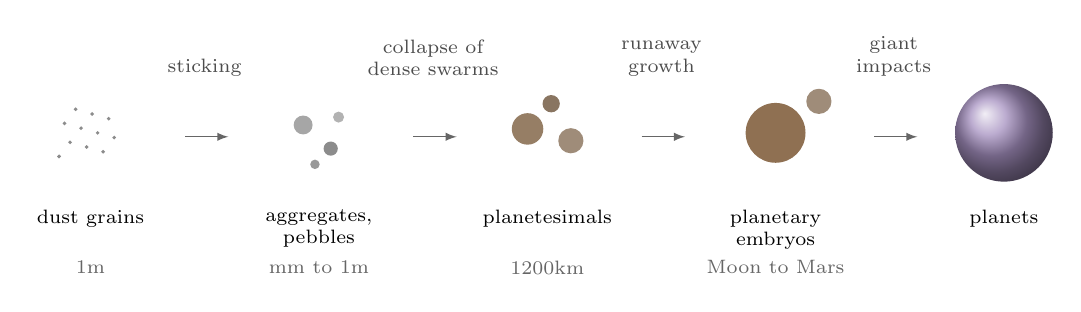
\begin{tikzpicture}[x=1cm, y=1cm, font=\scriptsize]
\foreach \x/\t/\s in {0/{dust grains}/{\qty{1}{\micro m}},
  2.9/{aggregates,\\pebbles}/{mm to \qty{1}{m}},
  5.8/{planetesimals}/{\qtyrange{1}{200}{km}},
  8.7/{planetary\\embryos}/{Moon to Mars},
  11.6/{planets}/{} } {
  \node[align=center, anchor=north] at (\x,-0.9) {\t};
  \node[align=center, anchor=north, black!60] at (\x,-1.55) {\s};
}
\foreach \i in {0,...,11} {\fill[black!45] ({-0.4+0.07*mod(\i*7,11)},{-0.35+0.06*mod(\i*5,11)}) circle (0.025);}
\fill[black!35] (2.7,0.05) circle (0.12); \fill[black!45] (3.05,-0.25) circle (0.09);
\fill[black!40] (2.85,-0.45) circle (0.06); \fill[black!30] (3.15,0.15) circle (0.07);
\fill[brown!55!black!70] (5.55,0) circle (0.2); \fill[brown!50!black!60] (6.1,-0.15) circle (0.16);
\fill[brown!45!black!70] (5.85,0.32) circle (0.11);
\fill[brown!60!black!80] (8.7,-0.05) circle (0.38); \fill[brown!50!black!60] (9.25,0.35) circle (0.16);
\shade[ball color=blue!45!brown!60] (11.6,-0.05) circle (0.62);
\foreach \x in {1.2,4.1,7.0,9.95} {\draw[-latex, black!60] (\x,-0.1) -- +(0.55,0);}
\node[align=center, anchor=south, black!70] at (1.45,0.55) {sticking};
\node[align=center, anchor=south, black!70] at (4.35,0.55) {collapse of\\dense swarms};
\node[align=center, anchor=south, black!70] at (7.25,0.55) {runaway\\growth};
\node[align=center, anchor=south, black!70] at (10.2,0.55) {giant\\impacts};
\end{tikzpicture}

\par\smallskip{\small From dust to planets in the region of the rocky planets
(schematic, not to scale). Grains stick into aggregates; swarms of pebbles collapse
into \omterm{def:b2:planet-formation-meteorites:planetesimal}{planetesimals}; gravity makes some \omterm{def:b2:planet-formation-meteorites:planetesimal}{planetesimals} run away into embryos, which
end by merging into planets. Beyond the \omterm{def:b2:planet-formation-meteorites:snow-line}{snow line} the embryos grew larger and could
capture gas. Sizes from Chiang and Youdin (2010) and Lugaro and others (2018).}
% ledger: cy10:growth, lugaro:cai
\end{omfigure}

The planets kept little memory of this history: they melted, mixed and
reworked their matter. The record is in the bodies that stopped growing, the
asteroids, and in the pieces of them that reach the Earth.

\section{Meteorites}

\begin{definition}[Meteorite, meteorite fall, meteorite find]
\label{def:b2:planet-formation-meteorites:fall-find}
A \emph{meteorite}\index{meteorite} is a natural solid object from space that
has survived its passage through the atmosphere and reached the ground. A
\emph{meteorite fall}\index{meteorite fall} is a meteorite collected after its
arrival was observed, usually as a fireball; a \emph{meteorite
find}\index{meteorite find} is one recognised on the ground without its fall
having been seen.
\end{definition}

The Earth sweeps up far more dust than stones. Measured in the snow of the
Antarctic plateau, about \qty{5200}{t} of extraterrestrial dust reaches the
ground each year as micrometeorites and molten spherules, out of some
\qty{15000}{t} that enter the atmosphere, most of it shed by comets and about a
fifth by asteroids. \omterm{def:b2:planet-formation-meteorites:fall-find}{Meteorites}, the stones and irons large enough to be
recognised one by one, are fewer: the world's catalogue holds about
\num{45000} of them, of which only \num{1107} are falls.
% ledger: rojas21:flux, data:b4-meteorites

The distinction matters. A fall is collected within days, before rain and
oxygen have altered it, and every kind of \omterm{def:b2:planet-formation-meteorites:fall-find}{meteorite} that falls is collected
alike; a find may have lain on the ground for thousands of years, and its
chance of being found depends on how it looks and where it fell. Half of all
finds have been made in Antarctica (box below), where the search is
systematic. The falls are the fairer sample of what arrives (figure below):
more than four in five are \omterm{def:b2:planet-formation-meteorites:chondrule}{chondrites}, three in four ordinary \omterm{def:b2:planet-formation-meteorites:chondrule}{chondrites}.
% ledger: data:b4-meteorites

\begin{omfigure}
\begin{tikzpicture}
\begin{axis}[width=0.86\linewidth, height=6.3cm, ybar, bar width=7pt,
  xmin=0.4, xmax=9.6, ymin=0.1, ymax=200, ymode=log, log origin=infty,
  xtick={1,...,9}, xticklabels={ordinary, carbonaceous, enstatite, other chondrites,
    HED, other achondrites, iron, stony-iron, unclassified},
  x tick label style={font=\scriptsize, rotate=30, anchor=north east, inner sep=1pt},
  tick label style={font=\scriptsize}, label style={font=\small},
  ylabel={share of the sample (\%)}, legend pos=north east, xtick pos=bottom,
  legend style={font=\scriptsize, draw=black!30}, ymajorgrids, grid style={black!12}]
\addplot[fill=orange!70, draw=none] table[x=idx, y=falls_pct] {figdata/out/bachelor-2-meteorites-frac.dat};
\addlegendentry{falls (\num{1107})}
\addplot[fill=blue!45, draw=none] table[x=idx, y=finds_pct] {figdata/out/bachelor-2-meteorites-frac.dat};
\addlegendentry{finds (\num{44534})}
\end{axis}
\end{tikzpicture}

\par\smallskip{\small \omterm{def:b2:planet-formation-meteorites:fall-find}{Meteorites} by class, as a percentage of the falls and of the
finds (logarithmic scale); HED: howardites, eucrites and diogenites. Data: NASA
export of the Meteoritical Bulletin Database of The Meteoritical Society
(\num{45641} valid \omterm{def:b2:planet-formation-meteorites:fall-find}{meteorites}).}
% ledger: data:b4-meteorites
\end{omfigure}

\begin{inthefield}[Searching for meteorites on the blue ice]
\begin{minipage}[t]{0.6\linewidth}\vspace{0pt}
Most of the Antarctic ice sheet is white snow, but on about
\qty{1}{\percent} of its surface, where mountains block the flow of the ice,
some \qty{5}{cm} of ice is lost each year and bare blue ice shows. \omterm{def:b2:planet-formation-meteorites:fall-find}{Meteorites}
that fell on the snow upstream, over tens of thousands of years, are buried,
carried along in the ice and brought back to the surface where it wastes away:
the blue ice is a trap. Since systematic collecting began in the mid-1970s,
teams have recovered more than \num{30000} specimens from such fields, and in
the catalogue half of all finds come from south of \ang{60}\,S. The searchers
cross the ice in lines, on foot or on snowmobiles, and every stone found is
collected, however ordinary it looks, so that the collection is not biased
towards the striking ones. Each find is photographed where it lies, to record
its context, and given a field number; later it receives its official name, a
three-letter code for the ice field followed by the year of the season and a
serial number. In the curation laboratory the stones are chipped with
stainless-steel tools or cut dry with a band saw; \omterm{def:b2:planet-formation-meteorites:chondrule}{carbonaceous chondrites},
which may hold organic compounds, have had a cabinet of their own since 1978.
\end{minipage}\hfill
\begin{minipage}[t]{0.37\linewidth}\vspace{0pt}
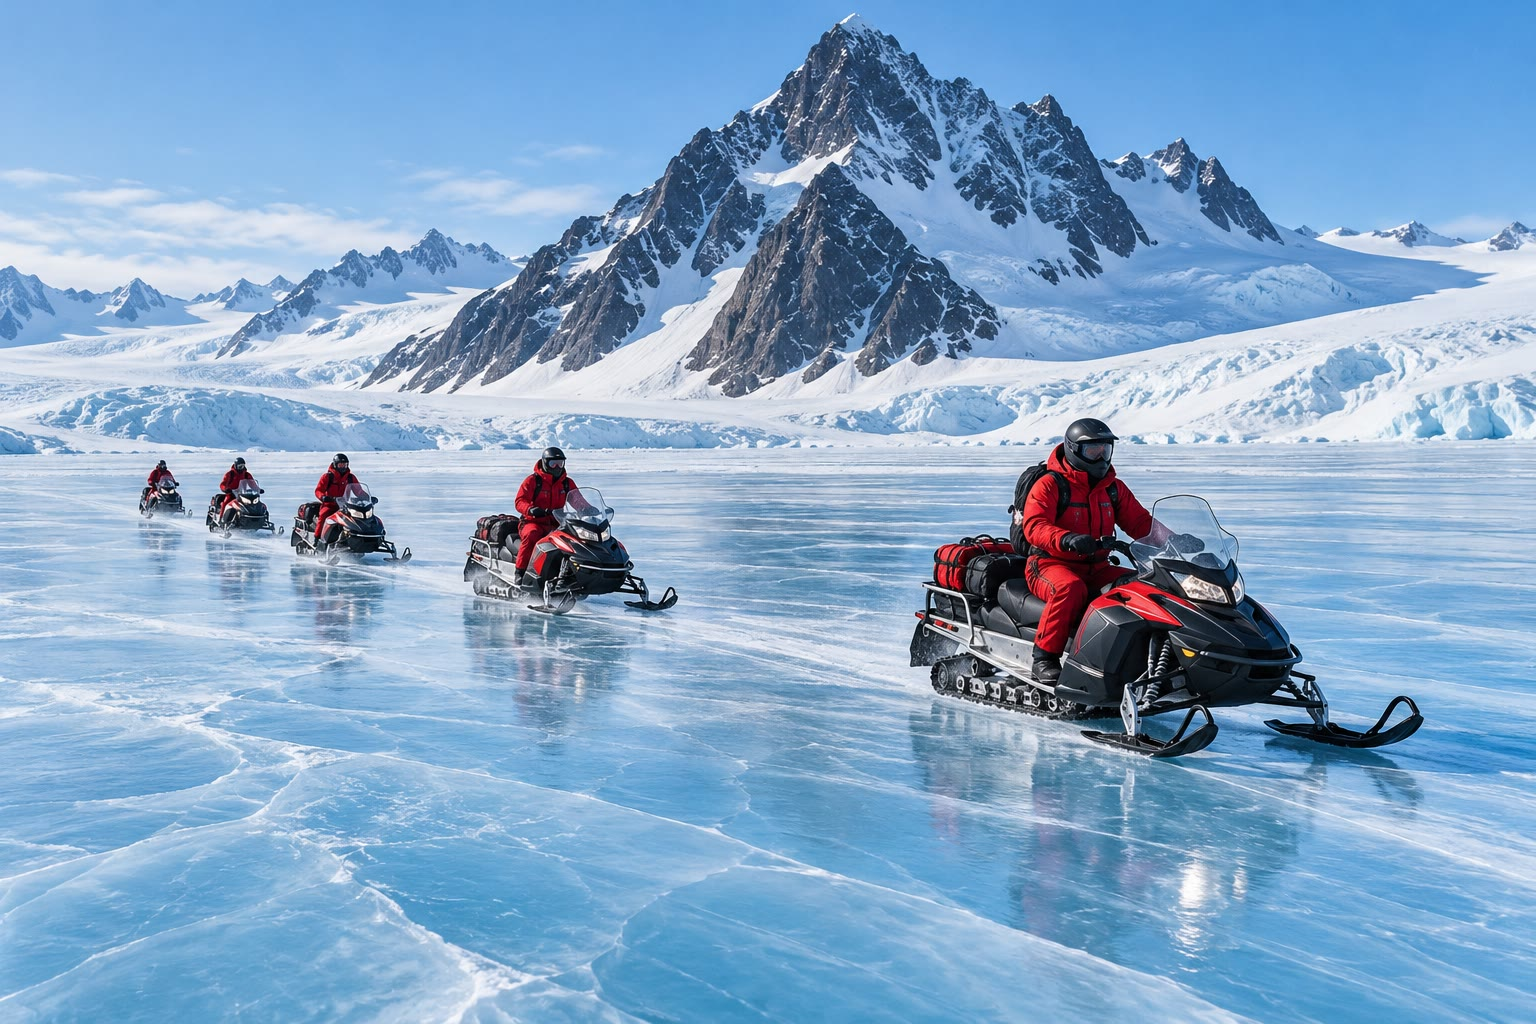
\includegraphics[width=\linewidth]{images/book4/ai/b2-blue-ice-search.jpg}

{\scriptsize A line of searchers on snowmobiles crossing a field of blue ice below
a rocky peak (AI-generated illustration).}
\end{minipage}
% ledger: folco06:blue-ice, data:b4-meteorites, nasa:antmet
\end{inthefield}

\subsection{Chondrites}

\begin{definition}[Chondrite, carbonaceous chondrite, chondrule, CAI]
\label{def:b2:planet-formation-meteorites:chondrule}
A \emph{chondrite}\index{chondrite} is a stony \omterm{def:b2:planet-formation-meteorites:fall-find}{meteorite} that never melted
after it was assembled, and whose composition, apart from the most volatile
elements, is close to that of the Sun. Most of it is made of
\emph{chondrules}\index{chondrule}, rounded droplets, a tenth of a millimetre to
about a centimetre across, of silicate rock that solidified from a melt, set in
a fine-grained matrix with grains of iron--nickel metal and iron sulfide. Some
chondrites hold \emph{calcium--aluminium-rich inclusions}\index{calcium--aluminium-rich
inclusion} (CAIs), irregular white grains of the minerals of calcium, aluminium
and titanium that are the first condensates of the nebula. A
\emph{carbonaceous chondrite}\index{carbonaceous chondrite} is a chondrite rich
in carbon, water-bearing minerals and matrix, whose content of the volatile
elements comes closest to the Sun's.
\end{definition}

The \omterm{def:b2:planet-formation-meteorites:chondrule}{chondrules} were molten for only minutes and cooled over hours to
days: some brief, local flash heating in the nebula, whose cause is still
unknown, melted clumps of dust, which froze as droplets before they were swept
together with dust and metal into a \omterm{def:b2:planet-formation-meteorites:planetesimal}{planetesimal}. They fill up to \qty{90}{\percent} of the volume of the most
primitive \omterm{def:b2:planet-formation-meteorites:fall-find}{meteorites}. The CAIs make up from less than \qty{1}{\percent} of
ordinary \omterm{def:b2:planet-formation-meteorites:chondrule}{chondrites} to over \qty{10}{\percent} of some carbonaceous ones, and they
formed within about a hundred thousand years of one another.
% ledger: gail:meteorites, cy10:growth, cy10:chondrules, gail:chondrite-table, lugaro:cai

\begin{omfigure}
\begin{minipage}[c]{0.5\linewidth}
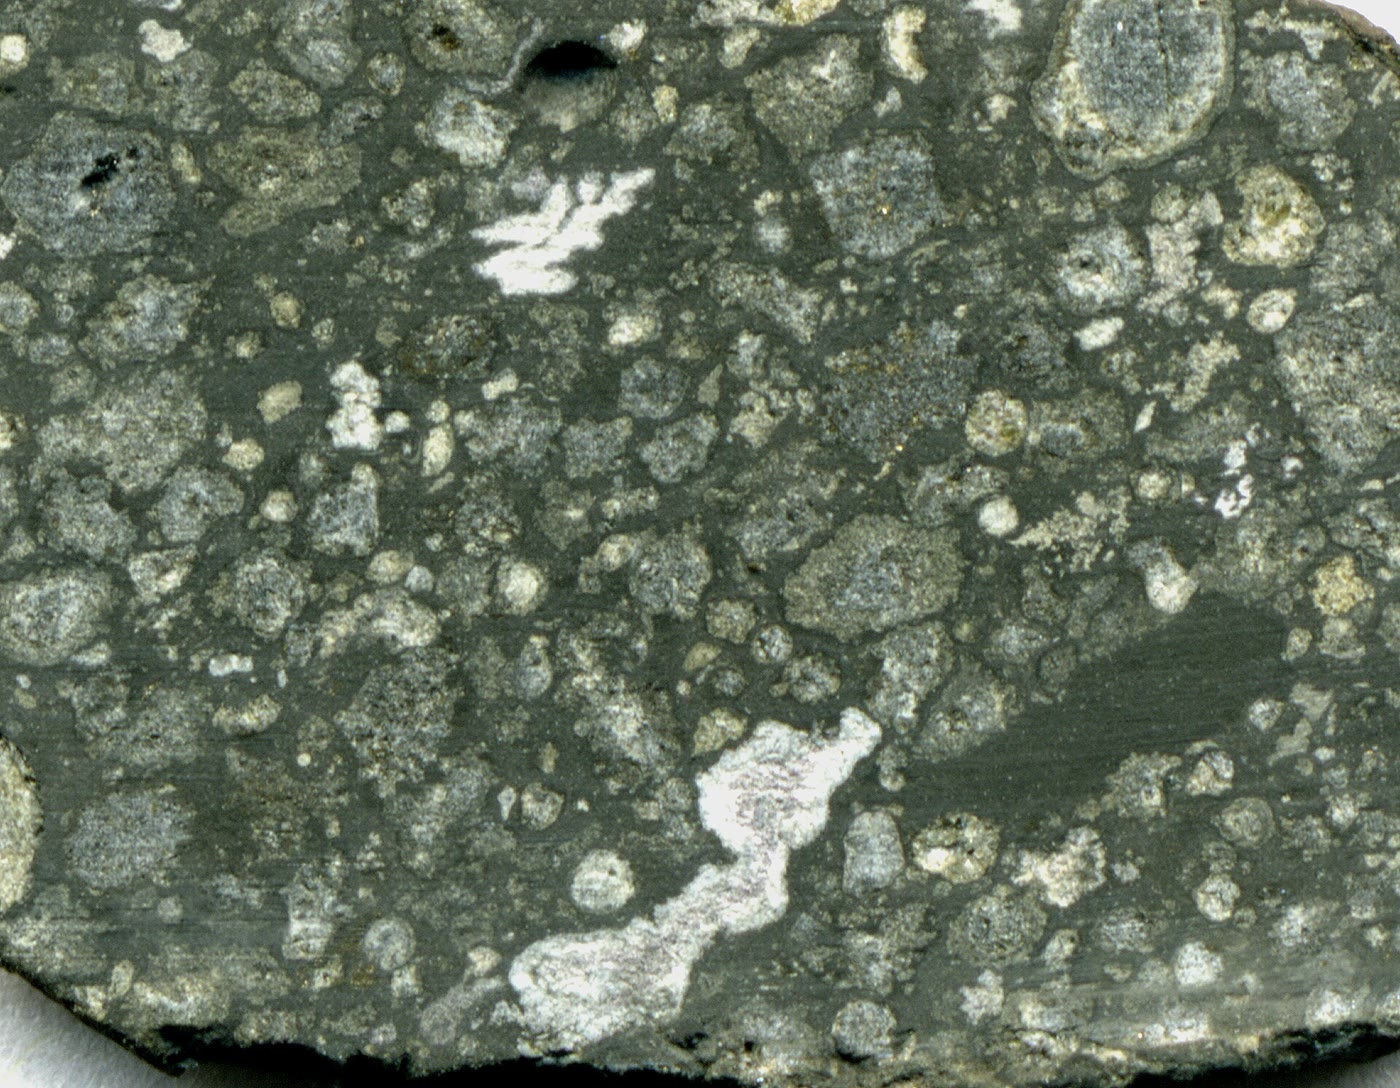
\includegraphics[width=\linewidth]{images/book4/b2-allende-chondrite.jpg}
\end{minipage}\hfill
\begin{minipage}[c]{0.46\linewidth}
{\small A cut face of the Allende \omterm{def:b2:planet-formation-meteorites:chondrule}{carbonaceous chondrite} (class CV3), which fell in
northern Mexico in 1969: about two tonnes were collected. The rounded grey grains are
\omterm{def:b2:planet-formation-meteorites:chondrule}{chondrules}; the irregular white patches are CAIs; the dark cement is the matrix. The
field is a few centimetres wide. James St.\ John, CC BY 2.0.}
\end{minipage}
% ledger: data:b4-meteorites, gail:chondrite-table
\end{omfigure}

\omterm{def:b2:planet-formation-meteorites:chondrule}{Chondrites} fall into groups that differ in the size and abundance of their
\omterm{def:b2:planet-formation-meteorites:chondrule}{chondrules}, their content of metal, the iron content of their olivine and the
proportion of their matrix (table below). The ordinary \omterm{def:b2:planet-formation-meteorites:chondrule}{chondrites} H, L and LL
have high, low and very low contents of metal and of total iron (atomic ratios
Fe/Si of \num{0.80}, \num{0.59} and \num{0.53}).
% ledger: gail:chondrite-table

\begin{table}[h]
\centering
\small
\begin{tabular}{lcccccc}
\hline
 & H & L & LL & CI & CM & CV\\
\hline
\omterm{def:b2:planet-formation-meteorites:chondrule}{chondrules} (vol.\ \%) & 60--80 & 60--80 & 60--80 & $\ll 1$ & 20 & 45\\
mean \omterm{def:b2:planet-formation-meteorites:chondrule}{chondrule} diameter (mm) & 0.3 & 0.7 & 0.9 & --- & 0.3 & 1.0\\
CAIs (vol.\ \%) & 0.1--1 & 0.1--1 & 0.1--1 & $\ll 1$ & 5 & 10\\
matrix (vol.\ \%) & 10--15 & 10--15 & 10--15 & $> 99$ & 70 & 40\\
iron--nickel metal (vol.\ \%) & 10 & 5 & 2 & 0 & 0.1 & 0--5\\
fayalite in olivine (mol \%) & 16--20 & 23--26 & 27--32 & & & \\
\omterm{def:b2:planet-formation-meteorites:type}{petrologic types} & 3--6 & 3--6 & 3--6 & 1 & 2 & 3\\
highest temperature (K) & 1220 & 1220 & 1220 & 430 & 670 & 870\\
\hline
\end{tabular}
\caption{Properties of the ordinary (H, L, LL) and of three \omterm{def:b2:planet-formation-meteorites:chondrule}{carbonaceous chondrite}
groups. Fayalite: the iron end-member of olivine. Data: Gail and others (2014).}
\label{tab:b2:planet-formation-meteorites:chondrites}
% ledger: gail:chondrite-table
\end{table}

\begin{definition}[Petrologic type]\label{def:b2:planet-formation-meteorites:type}
The \emph{petrologic type}\index{petrologic type} of a \omterm{def:b2:planet-formation-meteorites:chondrule}{chondrite} is a number
from 1 to 6 that records what happened to it in its parent body: type 3 is the
least altered; types 4 to 6 are increasingly heated, their \omterm{def:b2:planet-formation-meteorites:chondrule}{chondrules} blurred
and their minerals recrystallised and of uniform composition; types 2 and 1 are
increasingly altered by liquid water, which turned their minerals into clays.
\end{definition}

The last row of the table gives the highest temperatures reached by each group:
up to about \qty{1220}{K} for the most heated ordinary \omterm{def:b2:planet-formation-meteorites:chondrule}{chondrites}, never more
than \qty{430}{K} for the CI \omterm{def:b2:planet-formation-meteorites:chondrule}{chondrites}, soaked in water but never hot. The
heating, as the last section shows, came from inside the parent bodies.
% ledger: gail:chondrite-table

\subsection{Achondrites and irons}

\begin{definition}[Achondrite, iron meteorite, stony-iron meteorite]
\label{def:b2:planet-formation-meteorites:classes}
An \emph{achondrite}\index{achondrite} is a stony \omterm{def:b2:planet-formation-meteorites:fall-find}{meteorite} that crystallised
from a melt or recrystallised at high temperature in a body that melted, and
so has no \omterm{def:b2:planet-formation-meteorites:chondrule}{chondrules}. An \emph{iron meteorite}\index{iron meteorite} is made
mostly of iron--nickel metal. A \emph{stony-iron
meteorite}\index{stony-iron meteorite} is made of metal and silicate in roughly
equal amounts.
\end{definition}

These are the pieces of bodies that melted and separated: \omterm{def:b2:planet-formation-meteorites:classes}{achondrites} are their
crusts and mantles, irons their metal cores, and stony-irons come from where
metal and silicate met. The largest family of \omterm{def:b2:planet-formation-meteorites:classes}{achondrites}, the howardites,
eucrites and diogenites (HED), basalts and pyroxene-rich rocks, makes up
\qty{5.5}{\percent} of all falls. Its source was traced, by its spectrum and
its orbit, to the asteroid Vesta, about \qty{525}{km} across, and the Dawn
spacecraft, which reached Vesta in 2011, confirmed it: the chemistry
and mineralogy of Vesta's surface match the HED \omterm{def:b2:planet-formation-meteorites:fall-find}{meteorites}, a basin
\qty{500}{km} wide near its south pole shows where the fragments were knocked
off, and its gravity field points to an iron core about \qty{225}{km} across.
Vesta melted, nearly or entirely, early in its history. Other \omterm{def:b2:planet-formation-meteorites:classes}{achondrites} come
from the Moon and from Mars. The \omterm{def:b2:planet-formation-meteorites:fall-find}{meteorites} in the collections appear to come
from about a hundred different parent bodies.
% ledger: data:b4-meteorites, nasa:vesta-dawn, gail:meteorites

\omterm{def:b2:planet-formation-meteorites:classes}{Iron meteorites} keep the record of how their cores cooled. A cut and
acid-etched face shows a criss-cross of plates (figure below): at high
temperature the metal is a single alloy of iron and nickel; on slow cooling, a
nickel-poor alloy grows in plates along the planes of the original crystal,
and the slower the cooling, the wider the plates. Measured on many irons, the
plate widths give the cooling rates of the cores they came from.
% ledger: gail:meteorites

\begin{omfigure}
\begin{minipage}[c]{0.5\linewidth}
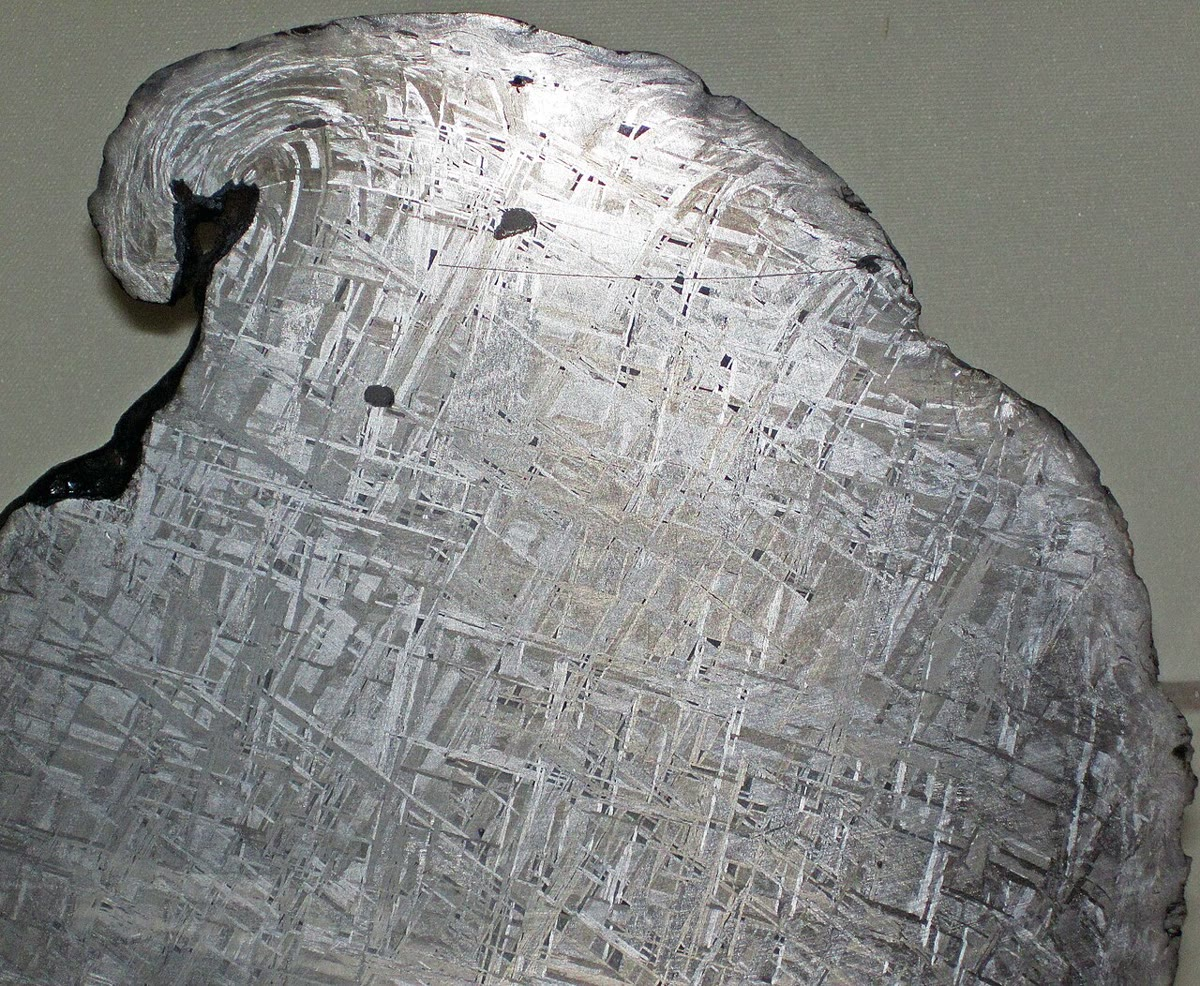
\includegraphics[width=\linewidth]{images/book4/b2-gibeon-widmanstatten.jpg}
\end{minipage}\hfill
\begin{minipage}[c]{0.46\linewidth}
{\small The cut, polished and acid-etched face of a piece of the Gibeon \omterm{def:b2:planet-formation-meteorites:classes}{iron meteorite},
found in Namibia: the criss-cross of plates of iron--nickel alloy (the Widmanstätten
pattern) grew as the metal core of its parent body cooled slowly. James St.\ John,
CC BY 2.0.}
\end{minipage}
% ledger: data:b4-meteorites
\end{omfigure}

\section{Dating the Solar System}

The age of the Solar System is the age of its oldest solids. Uranium--lead
isochrons of CAIs, built as in the Year 1 volume, give \qtyrange{4567}{4568}{\Ma};
the CAIs formed within about \qty{0.1}{Myr} of one another, a time short
enough for their age to be taken as the birth of the Sun. The events of the
next few million years, the formation of \omterm{def:b2:planet-formation-meteorites:chondrule}{chondrules} and the assembly and
melting of the first bodies, are best dated relative to the CAIs, with clocks
that ran fast and stopped early.
% ledger: lugaro:cai

\begin{definition}[Short-lived radionuclide]
\label{def:b2:planet-formation-meteorites:slr}
A \emph{short-lived radionuclide}\index{short-lived radionuclide} is a
radioactive nuclide with a half-life of roughly \num{0.1} to \qty{100}{Myr},
present when the Solar System formed and now extinct, whose former presence
is shown by an excess of its daughter in minerals that were rich in its
element.
\end{definition}

The best known is aluminium-26, which decays to magnesium-26 with a half-life of
\qty{0.717}{Myr} (a mean life of \qty{1.035}{Myr}). When the CAIs formed, one
aluminium atom in about \num{19000} was aluminium-26: the ratio
$\ce{^{26}Al}/\ce{^{27}Al}$ was $(5.23 \pm 0.13)\times10^{-5}$, the
\emph{canonical} value. Other short-lived nuclides cover longer spans (table
below).
% ledger: lugaro:al26, lugaro:slr-table

\begin{table}[h]
\centering
\small
\begin{tabular}{lllcc}
\hline
nuclide & daughter & reference & half-life (Myr) & early ratio\\
\hline
\ce{^{26}Al} & \ce{^{26}Mg} & \ce{^{27}Al} & 0.717 & $5.23\times10^{-5}$\\
\ce{^{60}Fe} & \ce{^{60}Ni} & \ce{^{56}Fe} & 2.62 & $1.0\times10^{-8}$\\
\ce{^{53}Mn} & \ce{^{53}Cr} & \ce{^{55}Mn} & 3.74 & $7\times10^{-6}$\\
\ce{^{107}Pd} & \ce{^{107}Ag} & \ce{^{108}Pd} & 6.5 & $6.6\times10^{-5}$\\
\ce{^{182}Hf} & \ce{^{182}W} & \ce{^{180}Hf} & 8.90 & $1.02\times10^{-4}$\\
\ce{^{129}I} & \ce{^{129}Xe} & \ce{^{127}I} & 15.7 & $1.28\times10^{-4}$\\
\hline
\end{tabular}
\caption{Some \omterm{def:b2:planet-formation-meteorites:slr}{short-lived radionuclides} of the early Solar System, their stable
daughter, the stable isotope of the same element used as reference, their
half-life and their ratio to the reference when the CAIs formed. Data: Lugaro and
others (2018).}
\label{tab:b2:planet-formation-meteorites:slr}
% ledger: lugaro:al26, lugaro:slr-table
\end{table}

\begin{proposition}[Relative age from an extinct nuclide]
\label{prop:b2:planet-formation-meteorites:relative-age}
If the ratio of a short-lived nuclide to its reference isotope was $R_0$
everywhere when the CAIs formed, and is found to have been $R$ in an object when
it formed, the object formed
\[
  \Delta t = \tau \ln\frac{R_0}{R}
\]
after the CAIs, where $\tau$ is the mean life of the nuclide. An error
$\delta R$ on $R$ gives the error $\tau\,\delta R/R$ on $\Delta t$.
\end{proposition}

\begin{proof}
The reference isotope is stable, so the ratio decays like the radioactive
nuclide itself: $R = R_0 e^{-\Delta t/\tau}$. Taking logarithms,
$\Delta t = \tau\ln(R_0/R)$. Differentiating, $\mathrm d(\Delta t) =
-\tau\,\mathrm dR/R$.
\end{proof}

A relative error of \qty{10}{\percent} on the ratio thus costs
\qty{0.1}{Myr} with aluminium-26 but \qty{0.54}{Myr} with manganese-53 and
\qty{1.3}{Myr} with hafnium-182: each clock is precise only over a few of its
own mean lives, and the right clock depends on the event. The ratio $R$ in an
object is read from its minerals.
% ledger: lugaro:al26, lugaro:slr-table

\begin{proposition}[Aluminium--magnesium isochron]
\label{prop:b2:planet-formation-meteorites:al-mg}
Let several minerals of one object form together at the time $\Delta t$ with the
same isotopic composition of magnesium, $(\ce{^{26}Mg}/\ce{^{24}Mg})_0$, but
different ratios $\ce{^{27}Al}/\ce{^{24}Mg}$, and stay closed since. Today they
lie on the straight line
\[
  \frac{\ce{^{26}Mg}}{\ce{^{24}Mg}}
  = \left(\frac{\ce{^{26}Mg}}{\ce{^{24}Mg}}\right)_0
  + R\,\frac{\ce{^{27}Al}}{\ce{^{24}Mg}},
\]
whose slope is the ratio $R = \ce{^{26}Al}/\ce{^{27}Al}$ of the object when it
formed.
\end{proposition}

\begin{proof}
Every aluminium-26 atom present at formation has since become a
magnesium-26 atom, so a mineral gained
$\ce{^{26}Al}_{\text{then}} = R\,\ce{^{27}Al}$ atoms of magnesium-26, aluminium-27
being stable. Dividing by the number of magnesium-24 atoms, which is unchanged,
gives the line.
\end{proof}

Aluminium-rich, magnesium-poor minerals such as plagioclase show large excesses
of magnesium-26; olivine, almost free of aluminium, shows none. This is how the
time sequence of the early Solar System was built: CAIs first; \omterm{def:b2:planet-formation-meteorites:chondrule}{chondrules} over
the following few million years, with the evidence from \omterm{def:b2:planet-formation-meteorites:chondrule}{chondrules} setting the
lifetime of the gas disc at less than five million years; the parent bodies of
the \omterm{def:b2:planet-formation-meteorites:chondrule}{chondrites} assembled after their youngest \omterm{def:b2:planet-formation-meteorites:chondrule}{chondrules}. The diogenites,
rocks of Vesta's mantle, began to crystallise within about a million years of
the CAIs, and Vesta's core formed within the first one to
four million years: \omterm{def:b2:planet-formation-meteorites:classes}{iron meteorites} and \omterm{def:b2:planet-formation-meteorites:classes}{achondrites} are older than many
\omterm{def:b2:planet-formation-meteorites:chondrule}{chondrites}.
% ledger: lugaro:cai, gail:vesta, gail:meteorites

\section{Heat from aluminium-26 and the first melting}

Where did the heat that melted Vesta, and metamorphosed the ordinary
\omterm{def:b2:planet-formation-meteorites:chondrule}{chondrites}, come from? Models and \omterm{def:b2:planet-formation-meteorites:fall-find}{meteorites} agree that in the earliest bodies
the dominant source was the decay of aluminium-26. In rock of chondritic composition it carried, at the start,
\qty{5}{MJ} per kilogram ready to be released within a few million years:
enough to heat the rock by thousands of kelvins, if the heat could not escape.
% ledger: lugaro:heat, lugaro:melting

\begin{proposition}[Heating of a planetesimal by aluminium-26]
\label{prop:b2:planet-formation-meteorites:heating}
Rock that receives the radioactive power $H_0 e^{-t/\tau}$ per kilogram, has
the specific heat capacity $c$ and loses no heat, warms after its accretion at
the time $t_a$ as
\[
  T(t) = T_0 + \frac{H_0\tau}{c}\left(e^{-t_a/\tau} - e^{-t/\tau}\right),
\]
and tends to the peak temperature
$T_{\max} = T_0 + (H_0\tau/c)\,e^{-t_a/\tau}$. A critical temperature
$T_c > T_0$ is reached only if the body accreted before
\[
  t_a^* = \tau\ln\frac{H_0\tau}{c\,(T_c - T_0)}.
\]
\end{proposition}

\begin{proof}
With no losses, $c\,\mathrm dT/\mathrm dt = H_0 e^{-t/\tau}$. Integrating from
$t_a$, where $T = T_0$, gives
$c\,(T - T_0) = H_0\tau\,(e^{-t_a/\tau} - e^{-t/\tau})$, which tends to
$H_0\tau e^{-t_a/\tau}$ as $t \to \infty$. Setting $T_{\max} = T_c$ and solving
for $t_a$ gives $t_a^*$; for an earlier accretion the peak is higher.
\end{proof}

A model of the parent body of the ordinary \omterm{def:b2:planet-formation-meteorites:chondrule}{chondrites} uses
$H_0 = \qty{1.9e-7}{W.kg^{-1}}$, $c = \qty{837}{J.kg^{-1}.K^{-1}}$ and
$T_0 = \qty{250}{K}$. Then $H_0\tau/c$ is about \qty{7400}{K}. Three
temperatures matter: near \qty{750}{K} the porous rock starts to sinter into a
compact one; near \qty{1200}{K} the metal and the iron sulfide begin to melt
together; near \qty{1700}{K} the last silicates melt. A body that accreted
before \qty{1.7}{Myr} melted entirely; before \qty{2.1}{Myr} its metal and sulfide
melted and could sink into a core; until about \qty{2.8}{Myr} it was at least
sintered and metamorphosed; later bodies stayed cool (figure below).
% ledger: gail:params, gail:temps, lugaro:al26

\begin{omfigure}
\begin{tikzpicture}
\begin{axis}[omrecord, name=left, width=0.45\linewidth, height=6.0cm,
  xmin=0, xmax=8, ymin=0, ymax=2300,
  xlabel={time after the CAIs (Myr)}, ylabel={temperature (K)},
  tick label style={font=\scriptsize}, label style={font=\small}]
\addplot[black!45, densely dashed, domain=0:8, samples=2] {750};
\addplot[black!45, densely dashed, domain=0:8, samples=2] {1200};
\addplot[black!45, densely dashed, domain=0:8, samples=2] {1700};
\addplot[thick, red!75!black] table[x=t_Myr, y=T_K] {figdata/out/bachelor-2-al26-ta15.dat};
\addplot[thick, orange!80!black] table[x=t_Myr, y=T_K] {figdata/out/bachelor-2-al26-ta20.dat};
\addplot[thick, teal!70!black] table[x=t_Myr, y=T_K] {figdata/out/bachelor-2-al26-ta25.dat};
\addplot[thick, blue!70!black] table[x=t_Myr, y=T_K] {figdata/out/bachelor-2-al26-ta30.dat};
\node[font=\tiny, red!75!black, anchor=south east] at (axis cs:7.9,1995) {$t_a = \qty{1.5}{Myr}$};
\node[font=\tiny, orange!80!black, anchor=south east] at (axis cs:7.9,1325) {2};
\node[font=\tiny, teal!70!black, anchor=south east] at (axis cs:7.9,915) {2.5};
\node[font=\tiny, blue!70!black, anchor=north east] at (axis cs:7.9,650) {3};
\node[font=\tiny, black!60, anchor=south west] at (axis cs:0.1,1700) {silicates melted};
\node[font=\tiny, black!60, anchor=south west] at (axis cs:0.1,1200) {Fe--FeS melts};
\node[font=\tiny, black!60, anchor=south west] at (axis cs:0.1,750) {sintering};
\end{axis}
\begin{axis}[omrecord, at={(left.east)}, anchor=west, xshift=2.1cm, width=0.45\linewidth,
  height=6.0cm, xmin=0, xmax=4, ymin=0, ymax=8000,
  xlabel={accretion time $t_a$ (Myr)}, ylabel={peak temperature (K)},
  tick label style={font=\scriptsize}, label style={font=\small},
  scaled y ticks=false, yticklabel style={/pgf/number format/1000 sep={\,}}]
\addplot[black!45, densely dashed, domain=0:4, samples=2] {750};
\addplot[black!45, densely dashed, domain=0:4, samples=2] {1200};
\addplot[black!45, densely dashed, domain=0:4, samples=2] {1700};
\addplot[thick, black] table[x=ta_Myr, y=Tpeak_K] {figdata/out/bachelor-2-al26-peak.dat};
\draw[black!60] (axis cs:1.69,0) -- (axis cs:1.69,1700);
\draw[black!60] (axis cs:2.13,0) -- (axis cs:2.13,1200);
\node[font=\tiny, black!70, anchor=south] at (axis cs:2.0,4500) {\qty{1.7}{Myr}};
\draw[black!50, -latex] (axis cs:2.0,4450) -- (axis cs:1.71,1800);
\node[font=\tiny, black!70, anchor=south] at (axis cs:2.9,3300) {\qty{2.1}{Myr}};
\draw[black!50, -latex] (axis cs:2.9,3250) -- (axis cs:2.16,1300);
\end{axis}
\end{tikzpicture}

\par\smallskip{\small Heating by aluminium-26 of the inside of a chondritic body with
no heat loss (the proposition above; $H_0 = \qty{1.9e-7}{W.kg^{-1}}$,
$c = \qty{837}{J.kg^{-1}.K^{-1}}$, $T_0 = \qty{250}{K}$, $\tau = \qty{1.035}{Myr}$).
Left: temperature against time for bodies accreted 1.5, 2, 2.5 and \qty{3}{Myr}
after the CAIs. Right: peak temperature against accretion time; bodies that accreted
before \qty{1.7}{Myr} melted, before \qty{2.1}{Myr} their metal and sulfide melted.
Real bodies spend part of the heat on melting, which caps the temperature, and lose
heat near their surface. Model values: Gail and others (2014).}
% ledger: gail:params, gail:temps, lugaro:al26
\end{omfigure}

The proposition ignores heat loss, which holds only deep inside a large body.
Heat diffuses over the distance $\sqrt{\kappa t}$ in the time $t$, where
$\kappa$ is the thermal diffusivity of the rock: with the values of the model,
about \qty{5}{km} in one mean life of aluminium-26 (\cref{exo:b2:planet-formation-meteorites:12}). Bodies much
smaller than this lose their heat as fast as they make it; detailed models show
that bodies more than \qtyrange{10}{20}{km} across could melt.
% ledger: gail:params, lugaro:melting

\begin{definition}[Planetary differentiation]
\label{def:b2:planet-formation-meteorites:differentiation}
\emph{Planetary differentiation}\index{planetary differentiation} is the
separation of a body, once molten or partly molten, into layers of different
composition and density: a metal core, a silicate mantle and a crust made of
the last melts.
\end{definition}

The \omterm{def:b2:planet-formation-meteorites:fall-find}{meteorites} thus record two kinds of early bodies. Those that formed within
about the first two million years had enough aluminium-26 to melt and
differentiate: their cores are the \omterm{def:b2:planet-formation-meteorites:classes}{iron meteorites}, their crusts and mantles
the \omterm{def:b2:planet-formation-meteorites:classes}{achondrites}, Vesta the survivor. Those that formed later stayed
\omterm{def:b2:planet-formation-meteorites:chondrule}{chondrites}, heated from inside to a degree set by their date of birth and by
the depth of each fragment: the deepest became type 6, the shallowest stayed
type 3. The Earth itself, built from embryos and \omterm{def:b2:planet-formation-meteorites:planetesimal}{planetesimals} of both kinds and
struck by giant impacts, differentiated into its core, mantle and crust.
% ledger: gail:meteorites, gail:vesta, gail:temps

\section{Exercises}

\begin{exercise}[$\star$]\label{exo:b2:planet-formation-meteorites:1}
In the minimum-mass \omterm{def:b2:planet-formation-meteorites:nebula}{solar nebula}, compute the surface density of the gas at
\qty{1}{au} and at \qty{5.2}{au}, and the surface density of the solids at
\qty{1}{au} (rock only, $Z_{\mathrm{rel}} = 0.33$) and at \qty{5.2}{au} (all ices
condensed, $Z_{\mathrm{rel}} = 1$). How many times heavier than the solids is the
gas at \qty{5.2}{au}?
% ledger: cy10:mmsn
\end{exercise}

\begin{exercise}[$\star$]\label{exo:b2:planet-formation-meteorites:2}
Using the figure of the \omterm{def:b2:planet-formation-meteorites:condensation}{condensation temperatures}, sort aluminium, sodium,
magnesium, iron, sulfur and oxygen (as water ice) from the first to condense to
the last, and give the volatility group of each. Which of them would you expect
to find enriched in CAIs, and which depleted in the Earth compared with the Sun?
% ledger: lodders:tc-table, lodders:groups
\end{exercise}

\begin{exercise}[$\star$]\label{exo:b2:planet-formation-meteorites:3}
The catalogue lists \num{1107} falls, of which 856 are ordinary \omterm{def:b2:planet-formation-meteorites:chondrule}{chondrites} and
49 irons, and \num{44534} finds, of which \num{38647} are ordinary \omterm{def:b2:planet-formation-meteorites:chondrule}{chondrites},
\num{1020} irons and \num{22096} come from south of \ang{60}\,S. Compute the
share of ordinary \omterm{def:b2:planet-formation-meteorites:chondrule}{chondrites} and of irons among the falls and among the finds,
and the share of Antarctic finds. Which sample would you use to estimate the
proportions in which the classes arrive on the Earth, and why?
% ledger: data:b4-meteorites
\end{exercise}

\begin{exercise}[$\star$]\label{exo:b2:planet-formation-meteorites:4}
The minerals of an object give the initial ratio
$\ce{^{26}Al}/\ce{^{27}Al} = \num{1.0e-5}$. How long after the CAIs did it form?
Take $R_0 = \num{5.23e-5}$ and a mean life of \qty{1.035}{Myr}.
% ledger: lugaro:al26
\end{exercise}

\begin{exercise}[$\star\star$]\label{exo:b2:planet-formation-meteorites:5}
Using \cref{prop:b2:planet-formation-meteorites:disc-mass} with
$\Sigma_1 = \qty{2.2e4}{kg.m^{-2}}$ at \qty{1}{au} (\qty{1}{au} $=
\qty{1.496e11}{m}$, $M_\odot = \qty{1.989e30}{kg}$), compute the mass of the
minimum-mass nebula inside \qty{30}{au} and inside \qty{100}{au}, in solar
masses. Compare with the observed discs, \numrange{0.001}{0.1} solar masses.
% ledger: cy10:mmsn
\end{exercise}

\begin{exercise}[$\star\star$]\label{exo:b2:planet-formation-meteorites:6}
In the passive disc $T = \qty{120}{K}\,(r/\qty{1}{au})^{-3/7}$, find where water
ice (\qty{182}{K}) and methane ice (\qty{41}{K}) become stable. A grain in direct
sunlight reaches \qty{182}{K} at \qty{2.3}{au}. Why do the two estimates of the
\omterm{def:b2:planet-formation-meteorites:snow-line}{snow line} differ, and which one applies to the bodies that built the planets?
% ledger: cy10:passive, lodders:phases
\end{exercise}

\begin{exercise}[$\star\star$]\label{exo:b2:planet-formation-meteorites:7}
Compute the isolation mass, with $b = 5$, of an embryo at \qty{1}{au} in the
minimum-mass nebula ($\Sigma_p = \qty{10.9}{g.cm^{-2}}$), and at \qty{5.2}{au}
beyond the \omterm{def:b2:planet-formation-meteorites:snow-line}{snow line} ($\Sigma_p = \qty{2.78}{g.cm^{-2}}$), in Earth masses
($M_\oplus = \qty{5.972e24}{kg}$, $M_\odot = \qty{1.989e30}{kg}$). What does it
become at \qty{5.2}{au} in a disc with \num{3.5} times more solids?
% ledger: cy10:isolation, cy10:mmsn, earth:mass
\end{exercise}

\begin{exercise}[$\star\star$]\label{exo:b2:planet-formation-meteorites:8}
Rock of CI composition held \num{1.01e16} atoms of aluminium-26 per gram when
the CAIs formed, and each decay leaves \qty{5.00e-13}{J} of heat. Compute the
heat released per kilogram over the whole decay, and the temperature rise it
would give with $c = \qty{837}{J.kg^{-1}.K^{-1}}$ and no losses. How many times
more is it than the heat needed to warm the rock from \num{250} to
\qty{1700}{K}?
% ledger: lugaro:heat, gail:params
\end{exercise}

\begin{exercise}[$\star\star$]\label{exo:b2:planet-formation-meteorites:9}
Over its whole decay, aluminium-26 releases \qty{5.07e10}{erg} per gram of CI
rock and iron-60 \qty{7.49e7}{erg} per gram. Compute the ratio of the two
energies. The half-life of iron-60 is \qty{2.62}{Myr}: compute its mean life,
and the ratio of the two initial heating powers, energy divided by mean life.
% ledger: lugaro:heat, lugaro:slr-table, lugaro:al26
\end{exercise}

\begin{exercise}[$\star\star\star$]\label{exo:b2:planet-formation-meteorites:10}
With the results of \cref{exo:b2:planet-formation-meteorites:9}, find the time after which iron-60 heats rock
faster than aluminium-26. Could iron-60 have melted a body that accreted that
late? (Compare the energy it still has to release then with the
\qty{1.2e6}{J.kg^{-1}} needed to warm rock from \num{250} to \qty{1700}{K}.)
% ledger: lugaro:heat, lugaro:slr-table, lugaro:al26
\end{exercise}

\begin{exercise}[$\star\star\star$]\label{exo:b2:planet-formation-meteorites:11}
With $H_0 = \qty{1.9e-7}{W.kg^{-1}}$, $\tau = \qty{1.035}{Myr}$,
$c = \qty{837}{J.kg^{-1}.K^{-1}}$ and $T_0 = \qty{250}{K}$ (a year of
\qty{3.156e7}{s}), compute the latest accretion times for which the centre of a
large body reaches \qty{1200}{K} and \qty{1700}{K}. Some measurements suggest that
the initial aluminium-26 was only half the canonical value in parts of the disc:
by how much would both times move? Show that the shift does not depend on the
critical temperature.
% ledger: gail:params, gail:temps, lugaro:al26
\end{exercise}

\begin{exercise}[$\star\star\star$]\label{exo:b2:planet-formation-meteorites:12}
Rock of conductivity \qty{2.1}{W.m^{-1}.K^{-1}}, density
\qty{3300}{kg.m^{-3}} and specific heat capacity \qty{837}{J.kg^{-1}.K^{-1}} has
the thermal diffusivity $\kappa = k/(\rho c)$. Compute it, and the distance
$\sqrt{\kappa\tau}$ over which heat diffuses in one mean life of aluminium-26.
Explain why the heating proposition applies to the centre of a body
\qty{100}{km} across but not to a body \qty{2}{km} across, and compare with the
smallest bodies that could melt, \qtyrange{10}{20}{km} across.
% ledger: gail:params, lugaro:melting, lugaro:al26
\end{exercise}

\section{Problem: The stone that fell on the frozen lake}

\begin{problem}[{Weekend problem --- classifying a freshly fallen stone, dating its
chondrules with aluminium-26, and finding how hot its parent body became}]
\label{pb:b2:planet-formation-meteorites:1}
% values: calc/ch02.py
% ledger: data:b4-meteorites, gail:chondrite-table, lugaro:al26, lugaro:cai, gail:params, gail:temps, cy10:mmsn, cy10:isolation, lodders:tc-table, earth:mass
On a winter night a fireball crosses the sky above an invented northern lake,
and a boom is heard. Next morning a black-crusted stone of \qty{2.4}{kg} is
picked up from the ice, in the middle of a fresh crater in the snow. The cut
stone shows \omterm{def:b2:planet-formation-meteorites:chondrule}{chondrules} making \qty{75}{\percent} of its volume, \qty{0.3}{mm}
across on average, with blurred edges; metal makes \qty{9}{\percent} of its
volume, and its olivine holds 18 mole per cent of fayalite. A laboratory
analyses one \omterm{def:b2:planet-formation-meteorites:chondrule}{chondrule} (table below). Use the tables of the chapter,
$R_0 = \num{5.23e-5}$, $\tau = \qty{1.035}{Myr}$, a year of \qty{3.156e7}{s},
$H_0 = \qty{1.9e-7}{W.kg^{-1}}$, $c = \qty{837}{J.kg^{-1}.K^{-1}}$,
$T_0 = \qty{250}{K}$, a conductivity of \qty{2.1}{W.m^{-1}.K^{-1}}, a density of
\qty{3300}{kg.m^{-3}}, \qty{1}{au} $= \qty{1.496e11}{m}$,
$M_\odot = \qty{1.989e30}{kg}$ and $M_\oplus = \qty{5.972e24}{kg}$.

\begin{center}
\small
\begin{tabular}{lcc}
\hline
mineral & $\ce{^{27}Al}/\ce{^{24}Mg}$ & $\ce{^{26}Mg}/\ce{^{24}Mg}$\\
\hline
olivine & 0.05 & \num{0.139500}\\
glass & 3.00 & \num{0.139518}\\
plagioclase & 15.0 & \num{0.139590}\\
\hline
\end{tabular}
\end{center}

\medskip
\noindent\textbf{Part I --- The stone.}
\begin{enumerate}
  \item Is the stone a fall or a find? Why does that make it valuable?
  \item Of the \num{1107} falls of the catalogue, 856 are ordinary \omterm{def:b2:planet-formation-meteorites:chondrule}{chondrites}. What
        is the chance that a fall, taken at random, is one?
  \item Using the table of \omterm{def:b2:planet-formation-meteorites:chondrule}{chondrite} groups, say to which group the stone belongs.
  \item Its \omterm{def:b2:planet-formation-meteorites:chondrule}{chondrules} have blurred edges and its minerals are of uniform
        composition. Which \omterm{def:b2:planet-formation-meteorites:type}{petrologic types} does that suggest, and what is the
        highest temperature its group reached, in kelvins and in degrees Celsius?
  \item Why would you expect few CAIs in it, and why is the stone nonetheless
        younger than any CAI?
\end{enumerate}

\noindent\textbf{Part II --- When did the chondrule form?}
\begin{enumerate}[resume]
  \item Explain why the ratio $\ce{^{26}Mg}/\ce{^{24}Mg}$ rises with
        $\ce{^{27}Al}/\ce{^{24}Mg}$ from mineral to mineral.
  \item From the olivine and the plagioclase, compute the slope of the isochron.
        What does it measure?
  \item Check that the glass lies on the same line.
  \item How long after the CAIs did the \omterm{def:b2:planet-formation-meteorites:chondrule}{chondrule} form?
  \item Taking the CAIs to be \qty{4567.5}{\Ma} old, give the age of the \omterm{def:b2:planet-formation-meteorites:chondrule}{chondrule}.
  \item What would the ratio $\ce{^{26}Al}/\ce{^{27}Al}$ have been in a mineral formed
        \qty{10}{Myr} after the CAIs? Which nuclide of the table would date such an
        event better?
\end{enumerate}

\noindent\textbf{Part III --- Heating the parent body.}
The stone's parent body, \qty{20}{km} in radius, assembled \qty{2.4}{Myr} after
the CAIs, soon after its \omterm{def:b2:planet-formation-meteorites:chondrule}{chondrules}.
\begin{enumerate}[resume]
  \item Compute the thermal diffusivity of the rock and the time $R^2/\kappa$ for
        heat to escape from the centre, in millions of years. May the centre be
        treated as losing no heat?
  \item Compute the heating power of aluminium-26 per kilogram of rock at the time
        of assembly.
  \item Compute the heat still to be released per kilogram after assembly.
  \item Compute the temperature rise and the peak temperature at the centre.
  \item Compare with the three critical temperatures of the chapter. Did the
        centre melt? Is this consistent with question 4?
  \item What is the latest assembly time for which the metal and sulfide of the
        centre would have begun to melt?
  \item How long after assembly is \qty{90}{\percent} of the temperature rise
        reached? Give the date after the CAIs.
\end{enumerate}

\noindent\textbf{Part IV --- The neighbours.}
\begin{enumerate}[resume]
  \item An \omterm{def:b2:planet-formation-meteorites:classes}{achondrite} comes from a body that assembled \qty{0.8}{Myr} after the
        CAIs. Compute the peak temperature that the proposition would give, and say
        what really happened to the body.
  \item How many times more aluminium-26 per kilogram did that body have at its
        assembly than the stone's parent body?
  \item The stone is poorer than the Sun in zinc and lead, but not in magnesium or
        aluminium. Use the \omterm{def:b2:planet-formation-meteorites:condensation}{condensation temperatures} to explain why.
  \item In the minimum-mass nebula, compute the surface density of rock
        ($Z_{\mathrm{rel}} = 0.33$) at \qty{2.5}{au}, where the parent body
        orbited.
  \item Compute the isolation mass at \qty{2.5}{au}, with $b = 5$, in kilograms and
        in Earth masses, and compare it with the mass of the parent body.
  \item State the peak temperature of the centre of the parent body, the key number
        of this problem, in degrees Celsius.
\end{enumerate}
\end{problem}
